% Provenance (never printed): cycle 2 "Questionner l'espace et le temps ---
% se situer dans l'espace": representations of familiar spaces (plans), "lire
% des plans, se reperer sur des cartes. Elements constitutifs d'une carte :
% titre, echelle, orientation, legende"; see sources/book1/PROVENANCE.md.
% Book 1, grade 2, chapter 2. Sync 1: "scale" is owned here; "cardinal
% directions" is the physics series' term (prose only); "compass rose" here.
\chapter{Van tekening tot kaart}\label{ch:g2:drawing-to-map}

Een duif vliegt over de school. Wat ziet ze? Niet de voordeuren, niet de
ramen, niet de gezichten van de kinderen: van daarboven ziet ze alleen de
bovenkant van de dingen. De daken van de gebouwen zijn grijze rechthoeken.
Het schoolplein is een grote lege vorm met een paar ronde boomkruinen. De
paden zijn dunne lijntjes. De duif ziet de school van bovenaf --- zoals een
\omterm{def:g2:drawing-to-map:map}{kaart} haar laat zien.

\begin{omfigure}
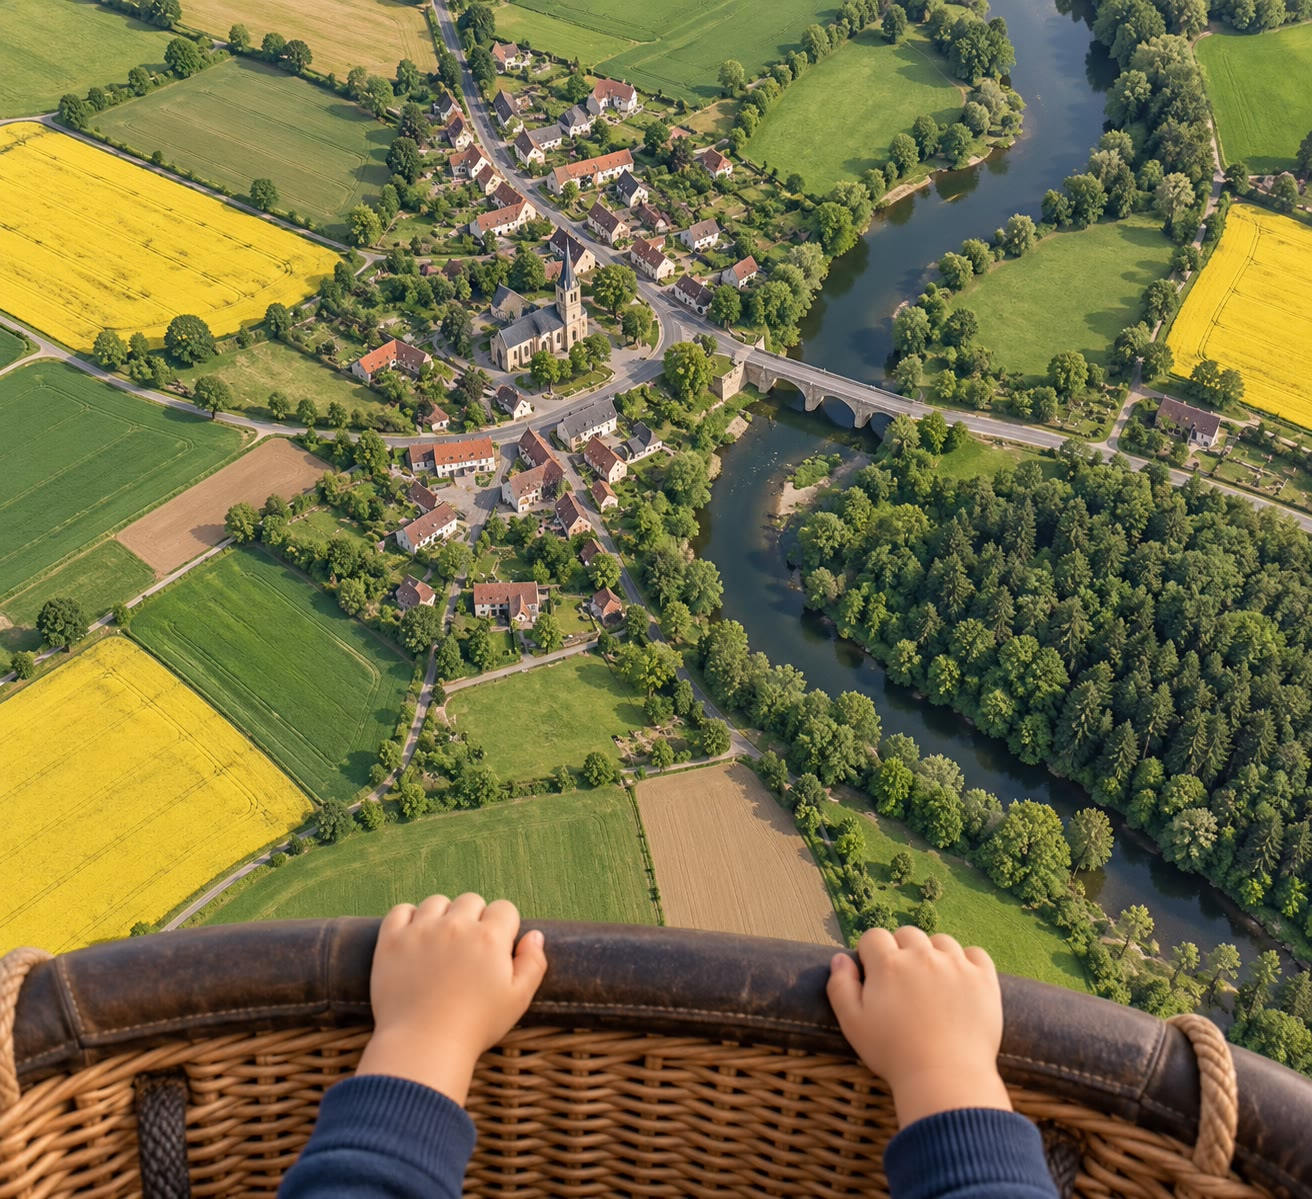
\includegraphics[width=0.62\linewidth]{images/book1/ai/g2-balloon-view.jpg}

{\small Het platteland gezien vanuit een luchtballon: akkers, een dorp, een
weg, een \omterm{def:g1:landscapes-around-us:water}{rivier} met een brug, alles van bovenaf gezien.}
\end{omfigure}

\section{Van opzij gezien, van bovenaf gezien}

Zet een paar speelgoedblokken op een tafel. Kijk er van opzij naar: je
ziet hoe hoog ze zijn, en de blokken achteraan worden verborgen door de
blokken vooraan. Ga nu staan en kijk er van bovenaf op neer: je ziet niet
meer hoe hoog ze zijn, maar je ziet precies waar elk blok staat en hoe ver
ze uit elkaar staan.

\begin{omfigure}
\begin{tikzpicture}[x=1cm, y=1cm, font=\small]
  % side view
  \begin{scope}
    \draw[black!50] (-0.2,0) -- (4.6,0);
    \fill[red!55, draw=black!60] (0.2,0) rectangle (1.2,1.6);
    \fill[ocBlue!55, draw=black!60] (1.6,0) rectangle (3.0,0.8);
    \fill[yellow!70, draw=black!60] (3.4,0) -- (3.9,1.1) -- (4.4,0) -- cycle;
    \node at (2.2,-0.5) {van opzij gezien};
  \end{scope}
  % from above
  \begin{scope}[shift={(6.4,0)}]
    \draw[black!30, fill=black!3] (-0.2,-0.1) rectangle (4.6,2.3);
    \fill[red!55, draw=black!60] (0.2,0.4) rectangle (1.2,1.4);
    \fill[ocBlue!55, draw=black!60] (1.6,1.0) rectangle (3.0,2.0);
    \fill[yellow!70, draw=black!60] (3.9,0.75) circle (0.5);
    \node at (2.2,-0.5) {van bovenaf gezien};
  \end{scope}
\end{tikzpicture}

{\small Drie blokken op een tafel: een hoog rood blok, een plat blauw blok
en een gele kegel. Van bovenaf is de kegel een cirkel en het hoge blok een
vierkant.}
\label{fig:g2:drawing-to-map:blocks}
\end{omfigure}

\begin{definition}[Plattegrond]\label{def:g2:drawing-to-map:plan}
Een \emph{plattegrond}\index{plattegrond} is een tekening van een kleine
plek --- een kamer, een huis, een school, een tuin --- zoals je die recht
van bovenaf ziet, kleiner getekend dan in het echt maar met elk deel op de
goede plaats.
\end{definition}

\section{Kleiner tekenen: de schaal}

Een klaslokaal is veel te groot om het zoals het is op een vel papier te
tekenen. We tekenen het kleiner --- maar elk deel moet op dezelfde manier
kleiner worden, anders klopt de \omterm{def:g2:drawing-to-map:plan}{plattegrond} niet. De makkelijkste manier is
ruitjespapier: één hokje op het papier staat voor één meter in het
klaslokaal.

\begin{definition}[Schaal]\label{def:g2:drawing-to-map:scale}
De \emph{schaal}\index{schaal} van een \omterm{def:g2:drawing-to-map:plan}{plattegrond} of een \omterm{def:g2:drawing-to-map:map}{kaart} vertelt
hoeveel kleiner de tekening is dan de echte plek: voor welke afstand op de
grond een lengte op de tekening staat. Bijvoorbeeld: \emph{1 hokje staat
voor 1 meter}.
\end{definition}

\begin{omfigure}
\begin{tikzpicture}[x=0.75cm, y=0.75cm, font=\scriptsize]
  \draw[black!15] (0,0) grid (10,8);
  \draw[black, line width=1.6pt] (0,0) rectangle (10,8);
  % board on the north wall
  \fill[black!70] (3,7.8) rectangle (7,8);
  % teacher's desk
  \fill[brown!50, draw=black!70] (4,6) rectangle (6,7);
  % pupils' desks: 3 rows of 3
  \foreach \x in {1,4,7} \foreach \y in {1,2.5,4}
    \fill[orange!45, draw=black!70] (\x,\y) rectangle ++(2,1);
  % cupboard
  \fill[ocBlue!40, draw=black!70] (9,5) rectangle (10,8);
  % door (gap) on the east wall, windows on the west wall
  \fill[white] (9.85,1) rectangle (10.15,2);
  \draw[black!70] (10,2) arc[start angle=90, end angle=180, radius=1];
  \foreach \y in {1.5,4.5}
    \draw[ocBlue, line width=2.5pt] (0,\y) -- (0,\y+2);
  % legend
  \begin{scope}[shift={(11,7.2)}]
    \node[anchor=west, font=\small\bfseries] at (0,0.4) {Het klaslokaal};
    \fill[black!70] (0,-0.25) rectangle (0.8,-0.05); \node[anchor=west] at (1,-0.15) {bord};
    \fill[brown!50, draw=black!70] (0,-1.1) rectangle (0.8,-0.7); \node[anchor=west] at (1,-0.9) {bureau van de leerkracht};
    \fill[orange!45, draw=black!70] (0,-1.85) rectangle (0.8,-1.45); \node[anchor=west] at (1,-1.65) {tafel van leerlingen};
    \fill[ocBlue!40, draw=black!70] (0,-2.6) rectangle (0.8,-2.2); \node[anchor=west] at (1,-2.4) {kast};
    \draw[ocBlue, line width=2.5pt] (0,-3.15) -- (0.8,-3.15); \node[anchor=west] at (1,-3.15) {raam};
    \draw[black!70] (0.8,-3.95) arc[start angle=0, end angle=90, radius=0.6]; \draw[black, line width=1.6pt] (0.2,-3.95) -- (0.8,-3.95); \node[anchor=west] at (1,-3.7) {deur};
    \draw[black!15] (0,-4.9) rectangle (0.75,-4.15);
    \node[anchor=west] at (1,-4.53) {1 hokje = 1 meter};
    \pic[scale=0.7, transform shape] at (0.7,-6.2) {compassrose};
  \end{scope}
\end{tikzpicture}

{\small De \omterm{def:g2:drawing-to-map:plan}{plattegrond} van een klaslokaal op ruitjespapier, met een titel,
een \omterm{def:g2:drawing-to-map:legend}{legenda}, een \omterm{def:g2:drawing-to-map:scale}{schaal} en een \omterm{def:g2:drawing-to-map:directions}{windroos}. De noordmuur, met het bord, ligt
bovenaan.}
\label{fig:g2:drawing-to-map:classroom}
\end{omfigure}
% (exercise data: an invented classroom of 10 m by 8 m)

\begin{method}[Meten op een plattegrond]\label{met:g2:drawing-to-map:measure}
Zo vind je een echte lengte op een \omterm{def:g2:drawing-to-map:plan}{plattegrond} die op hokjes is getekend:
\begin{enumerate}
  \item tel de hokjes langs de lengte die je wilt weten;
  \item lees de \omterm{def:g2:drawing-to-map:scale}{schaal}: voor hoeveel staat één hokje?
  \item geef het antwoord in meters (of op een \omterm{def:g2:drawing-to-map:map}{kaart} in kilometers).
\end{enumerate}
\end{method}

\begin{example}[Hoe lang is het klaslokaal?]\label{ex:g2:drawing-to-map:length}
Langs de noordmuur van de \omterm{def:g2:drawing-to-map:plan}{plattegrond} liggen 10 hokjes. Eén hokje staat
voor 1 meter, dus het klaslokaal is 10 meter lang. Langs de westmuur liggen
8 hokjes: het is 8 meter breed. Het bord beslaat 4 hokjes van de noordmuur:
het is 4 meter lang.
\end{example}

\begin{omfigure}
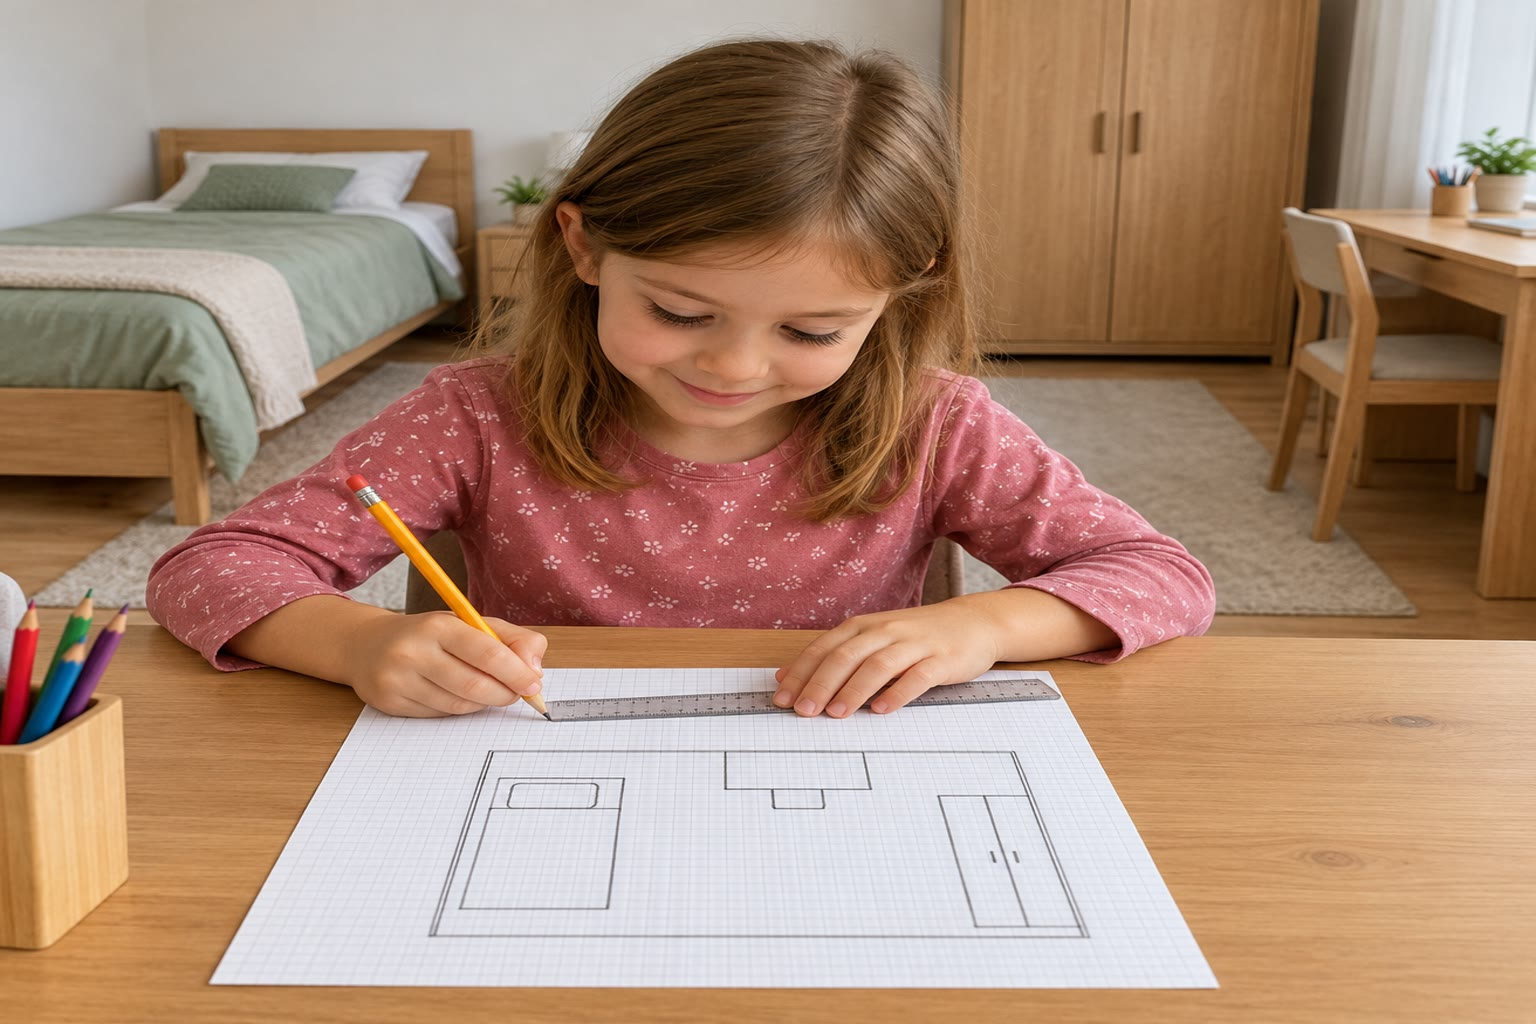
\includegraphics[width=0.55\linewidth]{images/book1/ai/g2-bedroom-plan.jpg}

{\small De \omterm{def:g2:drawing-to-map:plan}{plattegrond} van een slaapkamer tekenen op ruitjespapier.}
\end{omfigure}

\section{Van plattegrond tot kaart}

Een \omterm{def:g2:drawing-to-map:plan}{plattegrond} laat een kleine plek zien. Als we een grotere plek tekenen
--- een hele stad, een \omterm{def:g1:landscapes-around-us:landform}{dal}, een land --- dan tekenen we een \omterm{def:g2:drawing-to-map:map}{kaart}.

\begin{definition}[Kaart]\label{def:g2:drawing-to-map:map}
Een \emph{kaart}\index{kaart} is een tekening van een groot stuk van het
oppervlak van de Aarde, van bovenaf gezien en veel kleiner getekend dan het
in het echt is.
\end{definition}

Op een \omterm{def:g2:drawing-to-map:map}{kaart} is een huis veel te klein om te tekenen zoals het echt is.
Daarom gebruiken kaartenmakers kleine tekentjes: een stip voor een
boerderij, een blauwe lijn voor een \omterm{def:g1:landscapes-around-us:water}{rivier}, een groene vlek voor een bos.
Wat elk teken betekent, staat in een kader naast de \omterm{def:g2:drawing-to-map:map}{kaart}.

\begin{definition}[Legenda]\label{def:g2:drawing-to-map:legend}
Een \emph{kaartsymbool}\index{kaartsymbool} is een klein teken dat voor één
soort ding op een \omterm{def:g2:drawing-to-map:plan}{plattegrond} of een \omterm{def:g2:drawing-to-map:map}{kaart} staat. De
\emph{legenda}\index{legenda} is het kader dat elk symbool van de \omterm{def:g2:drawing-to-map:map}{kaart}
laat zien, met wat het betekent.
\end{definition}

\section{De weg vinden: de vier windrichtingen en de windroos}

Om te zeggen waar iets is, is ``links'' of ``rechts'' niet genoeg: wat
links van jou is, is rechts van iemand die tegenover je staat. Daarom
gebruiken mensen vier richtingen die voor iedereen hetzelfde zijn: noord,
oost, zuid en west. Je kent ze uit de natuurkundeboeken, van het kompas.
's Ochtends komt de Zon op in het oosten en 's avonds gaat ze onder in het
westen; noord en zuid liggen er precies tussenin, tegenover elkaar.

\begin{omfigure}
\begin{tikzpicture}[font=\small]
  \pic[scale=1.5, transform shape] at (0,0) {compassrose};
  \node[align=left, anchor=west, font=\small] at (2.6,0.3)
    {N = noord (bovenaan de meeste kaarten)\\O = oost (rechts)\\Z = zuid (onderaan)\\W = west (links)};
\end{tikzpicture}

{\small Een \omterm{def:g2:drawing-to-map:directions}{windroos}. Tussen noord en oost ligt het noordoosten; tussen
zuid en west het zuidwesten.}
\label{fig:g2:drawing-to-map:rose}
\end{omfigure}

\begin{definition}[Windroos]\label{def:g2:drawing-to-map:directions}
Een \emph{windroos}\index{windroos} is de ster op een \omterm{def:g2:drawing-to-map:map}{kaart} die de
richtingen noord, oost, zuid en west aangeeft. Op de meeste \omterm{def:g2:drawing-to-map:map}{kaarten} ligt
het noorden boven, het oosten rechts, het zuiden onder en het westen links.
\end{definition}

\begin{safety}
Kijk nooit naar de Zon om het oosten of het westen te vinden: je ogen
kunnen er voor altijd beschadigd door raken. Kijk liever naar de schaduwen,
of gebruik een kompas.
\end{safety}

\section{Een echte kaart lezen}

Elke goede \omterm{def:g2:drawing-to-map:map}{kaart} heeft vier onderdelen: een \textbf{titel} die zegt wat de
\omterm{def:g2:drawing-to-map:map}{kaart} laat zien, een \textbf{\omterm{def:g2:drawing-to-map:legend}{legenda}}, een \textbf{\omterm{def:g2:drawing-to-map:scale}{schaal}} en een
\textbf{\omterm{def:g2:drawing-to-map:directions}{windroos}} (of op zijn minst een pijl die naar het noorden wijst).
Hier is de \omterm{def:g2:drawing-to-map:map}{kaart} van een \omterm{def:g1:landscapes-around-us:landform}{dal} met \omterm{def:g1:landscapes-around-us:landform}{heuvels}, de Varden Hills. Het is een
verzonnen \omterm{def:g1:landscapes-around-us:landform}{dal} dat je in dit boek en in de volgende boeken steeds weer zult
tegenkomen, elke keer gedetailleerder getekend.

\begin{omfigure}
\begin{tikzpicture}
\begin{axis}[width=9.6cm, scale only axis,
    xmin=0, xmax=10, ymin=0, ymax=8, axis equal image,
    xtick={0,...,10}, ytick={0,...,8}, xticklabels={}, yticklabels={},
    grid=major, grid style={black!20}, major tick length=0pt,
    axis background/.style={fill=green!12!omLithAlluv},
    title={\textbf{De Varden Hills}}]
  \addplot[fill=omHypsLandD, draw=omHypsLandE!80!black, line width=0.4pt, fill opacity=0.85,
    unbounded coords=jump, even odd rule] table {figdata/out/grade-2-varden_plan-hills.dat};
  \addplot[fill=green!45!black!55, draw=green!35!black, line width=0.4pt] table {figdata/out/grade-2-varden_plan-wood.dat};
  \addplot[ocBlue!85!black, line width=2.2pt] table {figdata/out/shared-region-river.dat};
  \addplot[red!65!black, line width=1.3pt] table {figdata/out/grade-2-varden_plan-road.dat};
  \fill[black] (axis cs:5.012,3.414) ++(-3pt,-4pt) rectangle ++(6pt,8pt);
  \fill[white] (axis cs:5.012,3.414) ++(-1.6pt,-4pt) rectangle ++(3.2pt,8pt);
  \fill[brown!70!black] (axis cs:2.5,3.5) ++(-3.5pt,-3.5pt) rectangle ++(7pt,7pt);
  \fill[red!70!black] (axis cs:7.5,5.5) ++(-5pt,-3pt) rectangle ++(4pt,4pt);
  \fill[red!70!black] (axis cs:7.5,5.5) ++(1pt,-3pt) rectangle ++(4pt,4pt);
  \fill[red!70!black] (axis cs:7.5,5.5) ++(-2pt,2pt) rectangle ++(4pt,4pt);
\end{axis}
\begin{scope}[shift={(10.2,6.4)}, font=\small]
  \node[anchor=west, font=\small\bfseries] at (-0.1,0.55) {Legenda};
  \fill[omHypsLandD, draw=omHypsLandE!80!black] (0,-0.2) rectangle (0.7,0.15); \node[anchor=west] at (0.85,0) {heuvels};
  \fill[green!45!black!55] (0,-0.85) rectangle (0.7,-0.5); \node[anchor=west] at (0.85,-0.67) {bos};
  \draw[ocBlue!85!black, line width=2.2pt] (0,-1.35) -- (0.7,-1.35); \node[anchor=west] at (0.85,-1.35) {rivier};
  \draw[red!65!black, line width=1.3pt] (0,-2.0) -- (0.7,-2.0); \node[anchor=west] at (0.85,-2.0) {weg};
  \fill[black] (0.25,-2.8) rectangle (0.45,-2.5); \fill[white] (0.3,-2.8) rectangle (0.4,-2.5); \node[anchor=west] at (0.85,-2.65) {brug};
  \fill[brown!70!black] (0.23,-3.45) rectangle (0.47,-3.21); \node[anchor=west] at (0.85,-3.33) {boerderij};
  \foreach \dx/\dy in {0.12/-4.1, 0.33/-4.1, 0.22/-3.92}
    \fill[red!70!black] (\dx,\dy) rectangle ++(0.13,0.13);
  \node[anchor=west] at (0.85,-3.98) {dorp};
  \draw[black!40] (0,-4.95) rectangle (0.5,-4.45); \node[anchor=west, align=left] at (0.85,-4.7) {1 hokje\\= 1 kilometer};
  \pic[scale=0.75, transform shape] at (0.8,-6.5) {compassrose};
\end{scope}
\end{tikzpicture}

{\small Een eenvoudige \omterm{def:g2:drawing-to-map:map}{kaart} van de Varden Hills, met een titel, een
\omterm{def:g2:drawing-to-map:legend}{legenda}, een \omterm{def:g2:drawing-to-map:scale}{schaal} en een \omterm{def:g2:drawing-to-map:directions}{windroos}. De \omterm{def:g1:landscapes-around-us:water}{rivier} stroomt van west naar oost.}
\label{fig:g2:drawing-to-map:varden}
\end{omfigure}
% (figdata/grade-2/varden_plan.py; the region: figdata/shared/region.py)

\begin{method}[Een kaart lezen]\label{met:g2:drawing-to-map:read}
\begin{enumerate}
  \item Lees de titel: welke plek laat de \omterm{def:g2:drawing-to-map:map}{kaart} zien?
  \item Lees de \omterm{def:g2:drawing-to-map:legend}{legenda}: wat betekent elk symbool?
  \item Zoek de \omterm{def:g2:drawing-to-map:directions}{windroos}: waar is het noorden?
  \item Lees de \omterm{def:g2:drawing-to-map:scale}{schaal}, en tel hokjes om afstanden te vinden.
\end{enumerate}
\end{method}

\begin{example}[Van de boerderij naar het dorp]\label{ex:g2:drawing-to-map:farm}
Op de \omterm{def:g2:drawing-to-map:map}{kaart} van de Varden Hills ligt de boerderij ten zuiden van de \omterm{def:g1:landscapes-around-us:water}{rivier}.
Om naar het dorp te gaan, neemt de boer de weg naar het oosten, steekt de
\omterm{def:g1:landscapes-around-us:water}{rivier} over via de brug en gaat verder naar het noordoosten. Het dorp ligt
5 hokjes ten oosten van de boerderij en 2 hokjes ten noorden ervan: dat is
5 kilometer naar het oosten en 2 kilometer naar het noorden.
\end{example}

\section{Oefeningen}

\begin{exercise}[$\star$]\label{exo:g2:drawing-to-map:1}
Wordt een \omterm{def:g2:drawing-to-map:plan}{plattegrond} getekend zoals je iets van opzij ziet, of van bovenaf?
\end{exercise}

\begin{exercise}[$\star$]\label{exo:g2:drawing-to-map:2}
Wat is er op de \omterm{def:g2:drawing-to-map:plan}{plattegrond} van het klaslokaal in het blauw getekend bij de
westmuur? Wat staat er in de noordoostelijke hoek?
\end{exercise}

\begin{exercise}[$\star$]\label{exo:g2:drawing-to-map:3}
Noem de vier onderdelen die elke goede \omterm{def:g2:drawing-to-map:map}{kaart} moet hebben.
\end{exercise}

\begin{exercise}[$\star$]\label{exo:g2:drawing-to-map:4}
Welke richting ligt op de meeste \omterm{def:g2:drawing-to-map:map}{kaarten} bovenaan? Welke ligt links?
\end{exercise}

\begin{exercise}[$\star$]\label{exo:g2:drawing-to-map:5}
Op de \omterm{def:g2:drawing-to-map:plan}{plattegrond} van het klaslokaal beslaat een tafel van leerlingen
2 hokjes bij 1 hokje. Hoe lang en hoe breed is die tafel in het echte
klaslokaal?
\end{exercise}

\begin{exercise}[$\star$]\label{exo:g2:drawing-to-map:6}
Waar staat het bruine vierkantje op de \omterm{def:g2:drawing-to-map:map}{kaart} van de Varden Hills voor? En
de groene vlek?
\end{exercise}

\begin{exercise}[$\star\star$]\label{exo:g2:drawing-to-map:7}
Ligt het bos op de \omterm{def:g2:drawing-to-map:map}{kaart} van de Varden Hills ten noorden of ten zuiden van
de \omterm{def:g1:landscapes-around-us:water}{rivier}? Ligt het ten oosten of ten westen van de boerderij?
\end{exercise}

\begin{exercise}[$\star\star$]\label{exo:g2:drawing-to-map:8}
De hele \omterm{def:g2:drawing-to-map:map}{kaart} van de Varden Hills is 10 hokjes van west naar oost en
8 hokjes van zuid naar noord. Hoeveel kilometer is dat in elke richting?
\end{exercise}

\begin{exercise}[$\star\star$]\label{exo:g2:drawing-to-map:9}
Hoeveel tafels van leerlingen staan er op de \omterm{def:g2:drawing-to-map:plan}{plattegrond} van het
klaslokaal? Een leerling zit aan de tafel die het dichtst bij de deur
staat. Staat die in het noorden of in het zuiden van het klaslokaal?
\end{exercise}

\begin{exercise}[$\star\star$]\label{exo:g2:drawing-to-map:10}
Lucas tekent een \omterm{def:g2:drawing-to-map:plan}{plattegrond} van zijn slaapkamer. Zijn bed is 2 meter
lang. Hoeveel hokjes lang is het bed op zijn \omterm{def:g2:drawing-to-map:plan}{plattegrond}, met de \omterm{def:g2:drawing-to-map:scale}{schaal}
``1 hokje staat voor 1 meter''? Zijn slaapkamer is 4 meter lang en 3 meter
breed: hoeveel hokjes beslaat de hele kamer?
\end{exercise}

\begin{exercise}[$\star\star$]\label{exo:g2:drawing-to-map:11}
Lena zegt: ``De \omterm{def:g1:landscapes-around-us:water}{rivier} ligt links van mij.'' Waarom weten we dan nog niet
waar de \omterm{def:g1:landscapes-around-us:water}{rivier} ligt? Zeg het opnieuw op een manier die voor iedereen klopt,
als ze op de boerderij van de Varden Hills staat.
\end{exercise}
